% vim:tw=80 

\chapter{Introduction}

\section{About}
This document will explain how the Storage Performance Analyzer (SPA) can be used for
benchmarking. This guide starts with a high-level introduction of the architecture. Then, it includes the steps that are needed to set up the system under test as well as a step-by-step guide how to compile the tool, configure the benchmark that should be run, the actual benchmark, and the data retrieval using the R libraries.
This document concludes with a minimal running example with screenshots and a Q\&A section.

The web page of SPA is available at~\url{http://storageperformanceanalyzer.github.io/SPA/}. Publications describing the tool is available at~\cite{noorshams2013a,noorshams2014a}. 

\section{Requirements}

\textbf{Controller Machine:}
\begin{itemize}
  \item Platform independent (Windows, Unix and Mac operating systems tested) 
  \item Java 6 or later, Apache Ant for compilation 
  \item R version 3 or later (r-project.org) 
  \item SQLite version 3 (sqlite.org)
\end{itemize}

\textbf{System Under Test (SUT):}
\begin{itemize}
  \item POSIX compatible operating system (tested on Linux)  
  \item SSH access from the controller machine
\end{itemize}

\section{Download}

Platform-independent \emph{source code} as well as \emph{prepared drops} (i.e., already generated model code) for common operating systems both including \emph{examples} can be downloaded from the project web page~\url{http://storageperformanceanalyzer.github.io/SPA/}.

\chapter{Architecture}

\begin{figure}[htbp]
	\centering
	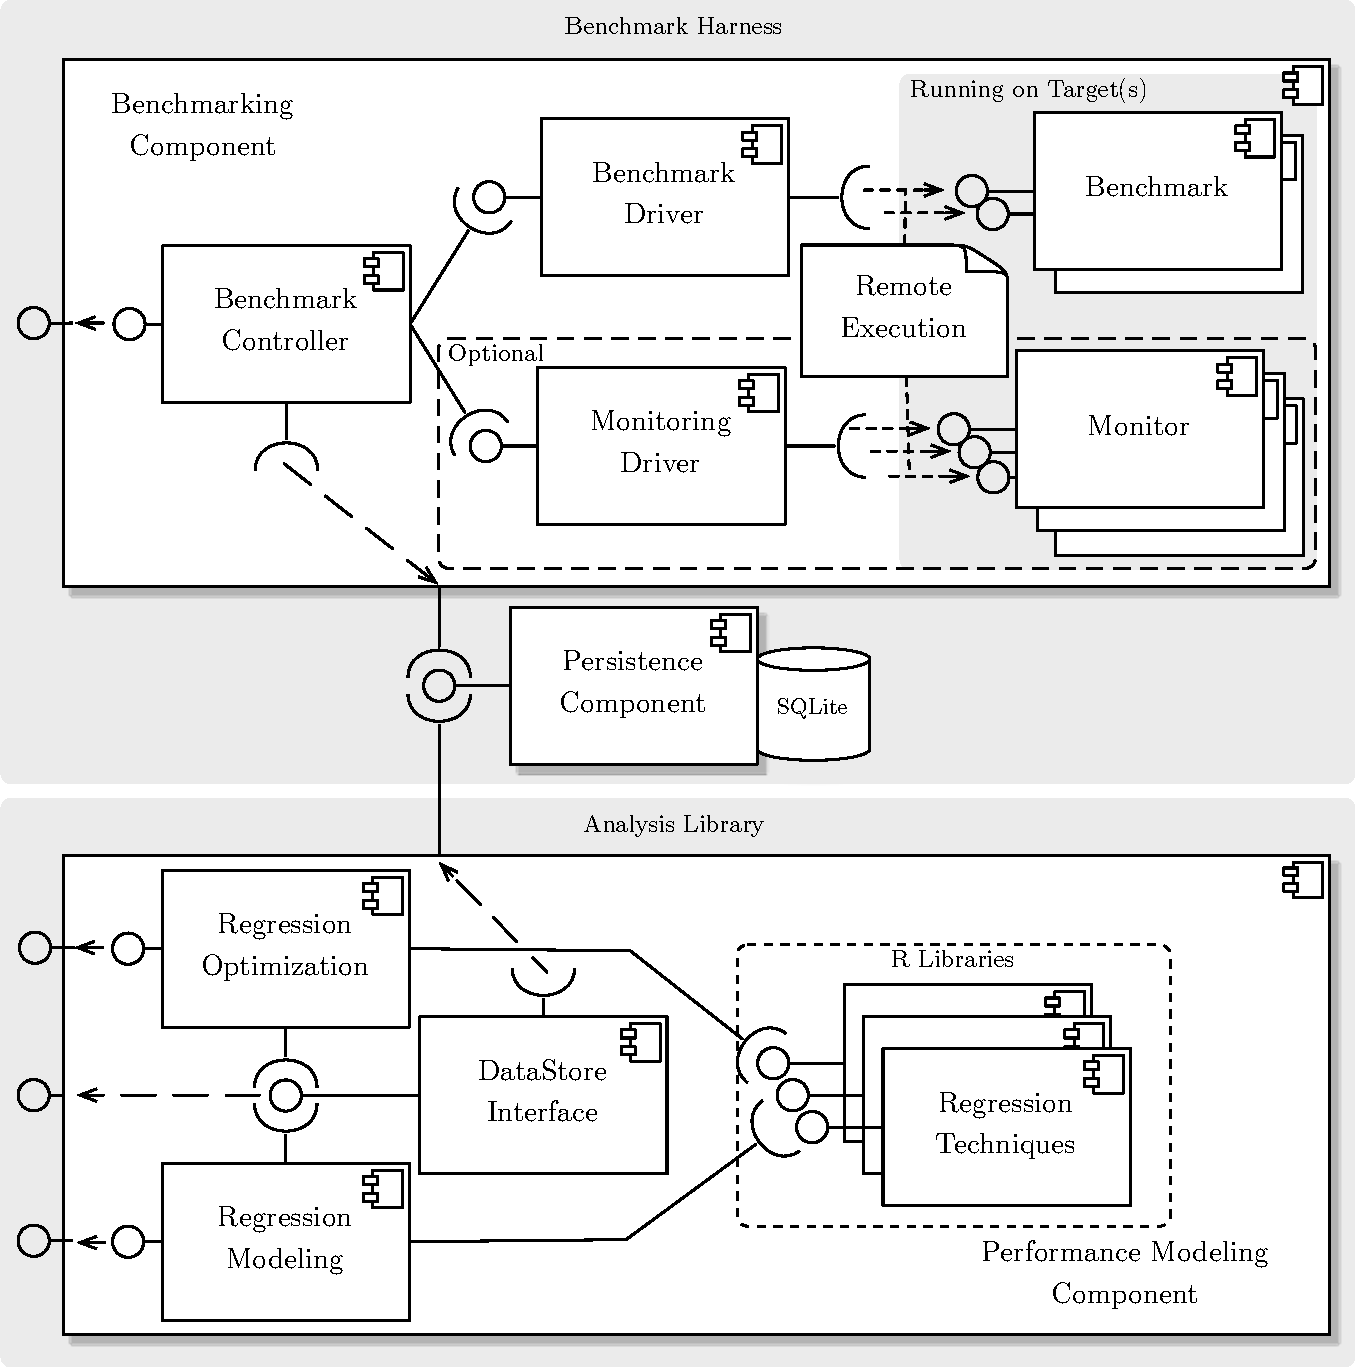
\includegraphics[scale=0.55]{graphics/Components.pdf}
	\caption{High-level Overview and Components of SPA}
 	\label{fig:ComponentDesign}
\end{figure}

Figure~\ref{fig:ComponentDesign} gives an high-level overview of SPA. The tool basically consists of a \textit{Benchmark Harness} and an \textit{Analysis Library}. The Benchmark Harness, which runs on a master machine, controls the parallel execution of benchmarks running on one or more remote targets (e.g., virtual machines). Furthermore, the benchmarking targets can be monitored using several self-composed or operating system monitors, e.g., \textit{blktrace}, where its \textit{Monitor Driver} already exists. The Analysis Library can be used to retrieve the measurements and use modeling functions to analyze the data and create regression models. 

\begin{figure}[htbp]
    \centering
    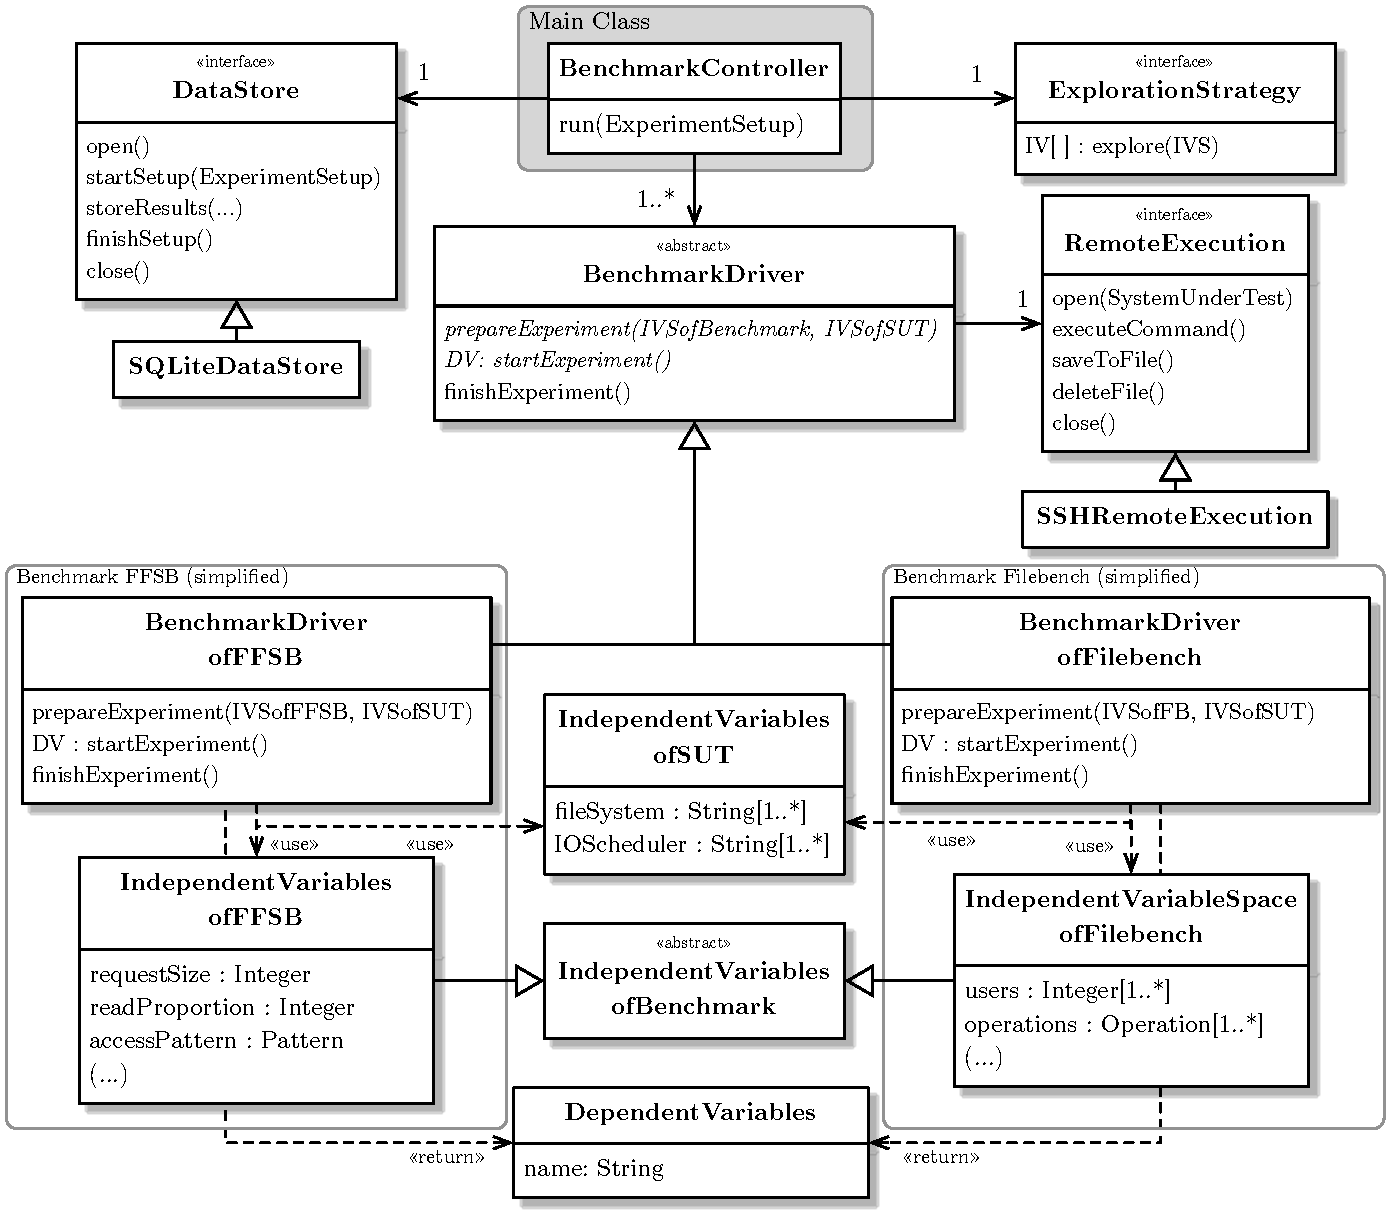
\includegraphics[scale=0.55]{graphics/Architecture.pdf}
    \caption{Most Important Classes of the Benchmark Harness}
    \label{fig:StaticDesign}
\end{figure}

The most important classes of the Benchmark Harness are shown in Figure~\ref{fig:StaticDesign}. The \textit{Benchmark Controller} is the main and core class. Also shown are how two specific benchmarks are integrated in the tool using a \textit{Benchmark Driver} and the respective configuration or \textit{Independent Variables}.

\begin{figure}[htbp]
    \centering
    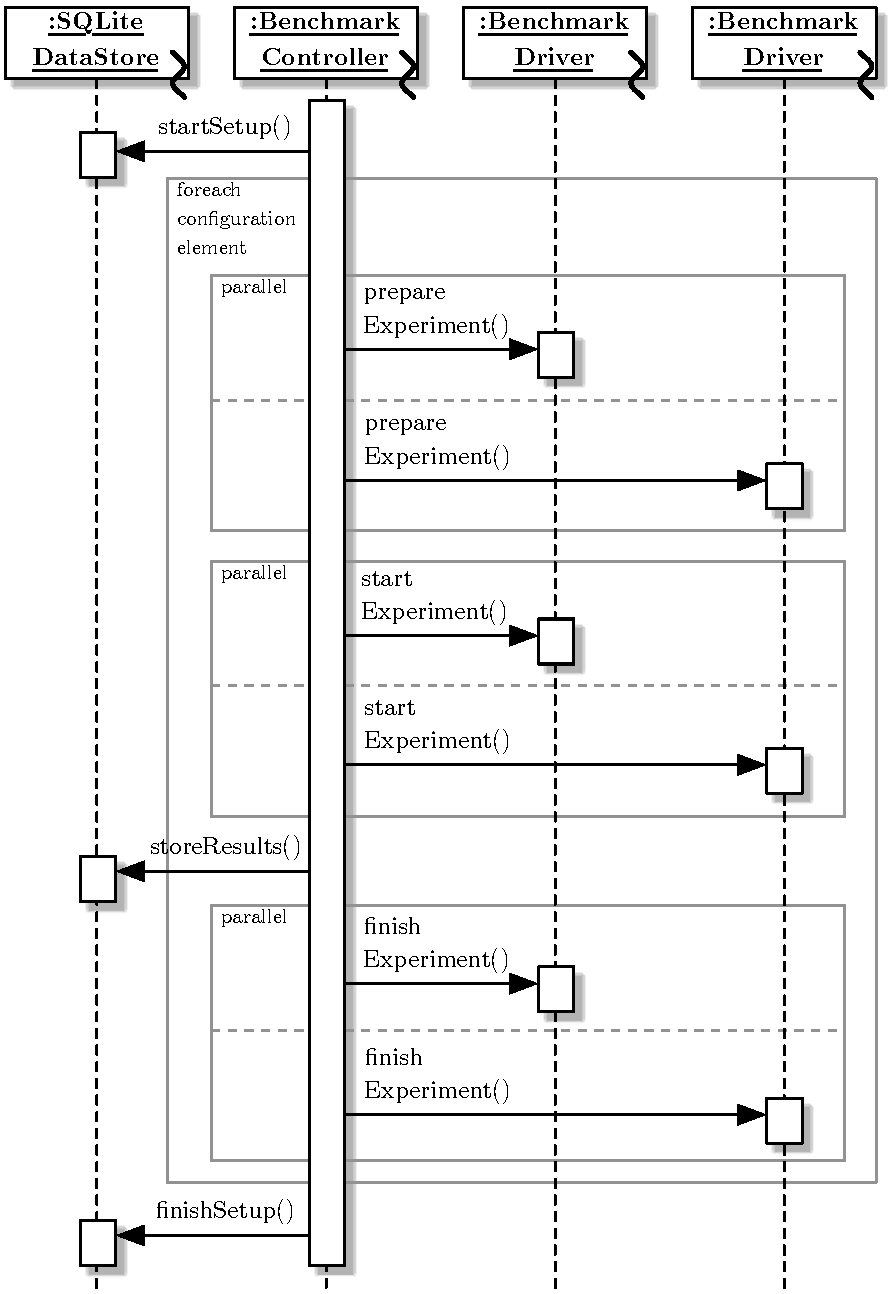
\includegraphics[scale=0.55]{graphics/BenchmarkSequence.pdf}
    \caption{Typical Benchmarking Sequence}
    \label{fig:BenchmarkingSequence}
\end{figure}

A typical benchmarking sequence with two targets (represented by the Benchmark Drivers) is shown in Figure~\ref{fig:BenchmarkingSequence}. The Benchmark Controller sets up the datastore and for every benchmark configuration element as explored by the \textit{Exploration Strategy} the measurements are started. The benchmark (or experiment) is prepared, started, and then finished. The results are stored to the datastore. The coordination is multi-threaded for a parallel execution of the benchmark and asynchronous data persistence.

\chapter{System Under Test Setup}
\label{sec:Setup}
Some manual steps are needed once on every system under test to set it up for
use together with the storage benchmark harness. The tool expects some
preconditions to be true. The following preconditions must be checked and met on
all systems under test.

\section{Authentication and Login}
\label{sec:usage_ssh_key}
The Storage Benchmark Harness must be able to connect to the machine and log in
using ssh. For this reason, a user which must have a shell and therefore be able
to login must exist. 

The authentication of the user is done using ssh keys. This method is a
alternative to ordinary passwords. It uses a public/private key pair where the
private key is only held by the client and the public key is stored on all
servers. Every client possessing the private key can connect to every server
where the public key is stored.

To generated a new key pair, the \texttt{ssh-keygen} application can be used.
This application is included in the default
OpenSSH\footnote{\url{http://openssh.org/}} distribution package. During the
creation of the key, no password may be specified. The Storage Benchmark Harness
relies on a key without a password because it has no abilities to ask for a
password during benchmarking.
If the user already has a public/private key pair, it can choose to either reuse this key
for the benchmarking or generate a second pair. The full path of the key should
be noted. The default path for the first key is typically
\texttt{\$\{HOME\}/.ssh/id\_rsa} but another path can be specified upon key
creation.

After a new key has been created or an existing key has been selected for reuse,
the key must be copied to all servers which will be involved in the
benchmarking. The can be done using the \texttt{ssh-copyid} command. A typical
call is \texttt{ssh-copyid -i \$\{HOME\}/.ssh/id\_rsa\_bench username@hostname}. 
An alternative is to copy the file manually if \texttt{ssh-copyis} is not available 
per default (like on Mac OS for example): 
\texttt{scp \$\{HOME\}/.ssh/id\_rsa\_bench.pub username@hostname:\$\{HOME\}/.ssh/authorized\_keys}.
During this copying the user has to specify the password which is set for the
user on the remote host. This command must be repeated for all hosts which will
be involved in the benchmarking.

To test whether the key generation has succeeded, the user can simply try to
connect to the remote host by using \texttt{ssh username@hostname -i \$\{HOME\}/.ssh/id\_rsa\_bench}. If the connection
succeeds without entering a password, the key was setup successfully.

For further documentation on the public/private keys see the man-pages of
\texttt{ssh}, \texttt{ssh-keygen} and \texttt{ssh-copyid}.
 
\section{Benchmark and Monitor Installation}
The benchmark must be installed on every system under test. Additionally its
executable must be in a directory which is included in the users \texttt{PATH}
variable. On a typical Linux installation, the \texttt{\$\{HOME\}/bin} directory
is already included in the path. If it is not, this can be achieved for one user 
by creating (or adjusting) the file \texttt{.bash\_profile} with the following 
lines: 
\begin{lstlisting}[language=bash]
  $ PATH=$PATH:${HOME}/bin
  $ export PATH
\end{lstlisting}
If this has to be changed system wide (except \emph{root}), those lines can be 
appended to the file \texttt{/etc/profile}.
The benchmark binaries can then be symlinked in the  \texttt{\$\{HOME\}/bin} 
directory for easier maintenance.

The monitoring tool \textsc{Blktrace} can be used and needs to be installed using the Linux tool \texttt{Aptitude}.

\subsection{Flexible File System Benchmark}
For the FFSB Benchmark, the Storage Benchmark Harness needs an extended version.
This version was forked from the original source and is available
online\footnote{\url{https://github.com/FFSB-Prime/ffsb}}. To
install FFSB and make it accessible for the Storage Benchmark Harness, the user
can use the following procedure after having logged in on the system under test:
\begin{lstlisting}[language=bash]
  $ cd ${HOME}
  $ svn co https://github.com/FFSB-Prime/ffsb
  $ # alternatively using git:
  $ # git clone https://github.com/FFSB-Prime/ffsb
  $ cd ffsb/trunk
  $ ./configure
  $ make
  $ ln -s  ${HOME}/ffsb/trunk/ffsb ${HOME}/bin/ffsb
\end{lstlisting}
The FFSB Benchmark driver must also modify files which are only writable by the
superuser. To achieve this, it uses the \texttt{sudo} command. Because the
Storage Benchmark Harness can not input passwords, the commands which need to be
executed using sudo must not ask for a password. Currently the only tool which
the storage benchmark harness must execute using sudo is the \texttt{tee}
command. In specific, the command is used to set or change the I/O scheduler as 
specified in the experiment configuration. To make the execution of this command 
password-less, edit the \textit{sudoers} file using \texttt{sudo visudo} and 
append the following line:
\begin{lstlisting}
ffsbTest ALL=NOPASSWD:/usr/bin/tee
\end{lstlisting}
Change \texttt{ffsbTest} to the appropriate user.

As for all storage benchmarks, the FFSB benchmarks needs a target directory
where the actual benchmarking should happen on the machine. Per default FFSB
used the \texttt{/tmp/ffsbtarget} directory on the system under test as target
directory. This directory was choosen because \texttt{/tmp} is writable by all
users. In this way a symlink can be used to select the actual target for ffsb.
For example, if the \texttt{/mnt/huge/target} directory should be used, the
following command creates the right symlink:
\begin{lstlisting}
   $ ln -s /mnt/huge/target /tmp/ffsbtarget
\end{lstlisting}
If for some reasons the directory which FFSB uses as target should be set
directly, this can be done by using the \texttt{ffsbtargetdir} environment
variable. 

The installation of the benchmark, the modification of the \textit{sudoers}
file and the symlinking of the target directory must be repeated for all systems
under test where a ffsb benchmark experiments should be executed.

\subsection{Filebench}
A bigfixed version of Filebench is available online\footnote{\url{https://github.com/Filebench-Revise}} and can be checked out using git. The user can take the following command 
to download the source code from the git-repository and install the benchmark:
\begin{lstlisting}[language=bash]
  $ cd ${HOME}
  $ git clone https://github.com/Filebench-Revise/Filebench-
    Revise.git filebench
  $ cd filebench
  $ ./configure
  $ make
  $ ln -s  ${HOME}/filebench ${HOME}/bin/filebench
\end{lstlisting}

As described in the FFSB Section the Filebench needs a directory to store its filesets. Filebench's default fileset location is
set to the \texttt{/tmp/filebenchtarget} directory on the system under test. Similar to FFSB a symlink can be used to point to a
different location (for example to \texttt{/mnt/huge/target}):
\begin{lstlisting}
   $ ln -s /mnt/huge/target /tmp/filebenchtarget
\end{lstlisting}
If for some reasons the directory which Filebench uses as target should be set
individually, this can be done by using the \texttt{filebenchtargetdir} environment
variable. Since filebench is restarted in case of an error, the following root rights are necessary, \texttt{echo} to obtain the process ID and \texttt{kill} to stop the process: 
\begin{lstlisting}
user ALL=NOPASSWD:/bin/echo
user ALL=NOPASSWD:/bin/kill
\end{lstlisting}

\subsection{Blktrace}
The Blktrace monitoring tool is usually part of the \texttt{sysstat} package and can be installed using the bash command:
\begin{lstlisting}
  $ apt-get update && apt-get install sysstat
  $ # sudo apt-get update && sudo apt-get install sysstat
\end{lstlisting}
The installation of the \texttt{sysstat} package requires root access. On some distributions, Blktrace has its own package, in that case replace \texttt{sysstat} with \texttt{blktrace} in the command.
  
Per default Blktrace records its results to the \texttt{/tmp/blktracetarget} directory on the system under test. As before the
location can be changed using a symlink:
\begin{lstlisting}
   $ ln -s /mnt/huge/target /tmp/blktracetarget
\end{lstlisting}
Alternatively it can be set by the help of the environment variable \texttt{blktracetargetdir}. 

Blktrace only runs with root rights. To post-process the monitoring files without root rights, the owner of the files created by Blktrace need to be changed to a normal user. This is achieved using the \texttt{changeOwner.sh} script that modifies the owner of the files to the owner of the respective parent folder. This avoids requiring root right for the \texttt{chown} command. The \texttt{changeOwner.sh}
script needs to be placed correctly and the execution attribute has to be set:
\begin{lstlisting}
   $ /usr/local/bin/changeOwner.sh
   $ chmod u+x /usr/local/bin/changeOwner.sh
\end{lstlisting}

Storage Benchmark Harness needs further root rights to allow a correct processing of all recording and analyzing steps. Thus, the
sudoers file has to be extended by the following lines:
\begin{lstlisting}
user ALL=NOPASSWD:/usr/sbin/blktrace
user ALL=NOPASSWD:/usr/local/bin/changeOwner.sh
user ALL=NOPASSWD:/bin/echo
user ALL=NOPASSWD:/bin/kill
\end{lstlisting}
Change \texttt{user} to the appropriate user. It is strongly recommended to use \texttt{sudo visudo} to modify the sudoers
file.

\chapter{Installation and Compilation}
\label{ch:Installation}
The Storage Benchmark Harness must be installed only on the measurement machine.
It needs an installed Java 6 JRE for running and a Java 6 SDK for compilation.
Additionally, Apache Ant\footnote{\url{http://ant.apache.org/}} must be
installed as build tool.

The source of the tool consists of two projects: The EMF\footnote{Eclipse
Modeling Framework} model (\textit{StorageBenchmarkHarnessModel}) and the actual
tool (\textit{StorageBenchmarkHarness}). When first using the tool, the two projects must be imported into an Eclipse with EMF Tools installed, e.g., using Eclipse Modeling Tools\footnote{\url{http://www.eclipse.org/downloads/packages/eclipse-modeling-tools/junosr1}}.
The code of the \textit{StorageBenchmarkHarnessModel} needs 
to be generated by using \texttt{SBHModel.genmodel} in the \texttt{model} folder. 
Simply open the file inside Eclipse and right-click on the \texttt{SBHModel} package and choose \texttt{Generate All}. The source can then be compiled by switching into the
\texttt{StorageBenchmarkHarness} folder and executing \texttt{ant}, e.g., using the shell/terminal. As all
libraries are included in the projects, the compilation should work without
further interaction. After this, the \texttt{run} binary in the folder should
work and display a help screen when executed using the shell\footnote{Tested on UNIX-based systems.}. Alternatively, the \texttt{main} method of \texttt{BenchmarkController} can be run inside Eclipse and the help message is shown on the console. Parameters can then be passed over the \texttt{run} configuration.

\chapter{Configuration}
After installing the tool, the next sections explain its configuration. For the
configuration of the tool, multiple pieces of information have to be specified:

\begin{itemize*}
    \item \textbf{\Gls{system under test}}: The connection information for each system
        under test must be configured. This includes the hostname, a user which
        can be used for logging and and a ssh-key which can be used for
        authentication.

    \item \textbf{\Glspl{experiment}}: The experiments which should be run on the hosts
        must be configured. This includes defining the independent variables by
        specifying independent variable spaces.

    \item \textbf{\Glspl{experiment series}}: The experiment series make the connection
        between a system under test and an independent variable spaces. It
        therefore defines which experiments should be executed on a system
        under test.

    \item \textbf{\Gls{experiment setup}}: The experiment setup contains multiple
        experiment series. In this way it contains the specification which
        experiments should be run on which hosts (In contrast to the experiment
        series which specifies which experiment should be run on \textit{one}
        host).
\end{itemize*}

These information can be either stored in a single configuration file or
distributed over multiple files for simpler reuse. The Storage Benchmark Harness
uses the Eclipse EMF Framework for the configuration file generation, editing
and parsing. The configuration files can be either edited by hand or using the
Eclipse EMF Tools.

\section{Eclipse Setup}
To use the EMF Tools, first Eclipse\footnote{\url{http://eclipse.org}} has to be
set up. The EMF Tools have to be installed together with eclipse either by
download a package which already includes the EMF or by later installing them.

The two projects which form the Storage Benchmark Harness can be imported into
eclipse as they are eclipse projects. This can be done by right-clicking in the
\textit{Package Explorer}, selecting {Import}, \textit{Existing Projects into
Workspace}. In the dialog the import can be finished by selecting the parent
directory (the directory containing the \texttt{StorageBenchmarkHarness} and
\texttt{StorageBenchmarkHarnessModel} directories). After the import as well as the 
code generation described in Section~\ref{ch:Installation}, the eclipse errors should 
go away after some seconds.

\section{Configuration File Creation}
\label{sec:configurationfilecreation}
To create a new configuration file using the EMF Tools, launch an eclipse instance in your eclipse or, more conveniently, install the plugins of the EMF model into your host eclipse. To do the latter, do the following (see \url{http://help.eclipse.org/juno/index.jsp?topic=%2Forg.eclipse.pde.doc.user%2Ftasks%2Fui_export_install_into_host.htm
}):
\begin{enumerate}
  \item Open the export wizard, either Open the plugin export wizard \emph{File > Export... > Plug-in Development > Deployable plug-ins and fragments}
  \item Select the plug-ins to export and install
  \item Select the last option on the Destination tab Install into host. Repository. Then choose a directory to create the repository in
  \item Hit Finish. The export operation will run followed by the installation operation.
  \item If the operations completed successfully, you will be prompted to restart. Choose to restart now
  \item Your plug-ins will be installed and running after the restart. You can see what has been installed using the Installation Details button on the About Dialog (available by going to Help > About Eclipse SDK)
\end{enumerate}

You will now be able to create instances of the configuration model using the wizard. Use \emph{File > New > Other... > Example EMF Model Creation Wizards > Configuration Model}. Choose destination and set \emph{Model Object} to \emph{Configuration}.  

As an \emph{alternative}, the following steps are possible as well \emph{in theory}:
\begin{enumerate*}
    \item Open the EMF Model in the
        \texttt{Storage\-Benchmark\-Harness\-Model\-/model\-/SBHModel\-.ecore} file using
        the \textit{ECore Model Editor}.
    \item Right click on the \textit{Configuration} EClass in the
        \textit{SBHModel}/\textit{Configuration} package. 
    \item Select \textit{Create Dynamic Instance}.
    \item Choose the filename and path for the configuration file and click on
        \textit{Finish}. 
    \item Open the newly created configuration file using the \textit{Reflective
        ECore Model Editor}. Due to a bug in EMF, the file get opened by the
        wrong editor by default.
\end{enumerate*}

\section{Referencing Configuration Fragments}
If the configuration is split in multiple configuration files, one configuration
file must reference instances from another configuration file. To include the
instances from other configuration files in the currently opened file, select
\textit{Reflective Editor} from the main menu of eclipse and then use the
\textit{Load Resource} functionality.


\section{Runnable Configuration Files}
The configuration model is shown in Figure~\ref{fig:DataModel}. Configuration files which 
will be used for the Storage Benchmark Harness must
include a \textit{Experiment Setup} child. This child contains all the
information which specifies multiple benchmark runs on multiple systems under
test. The actual specification can either be placed in the same configuration
file or be included from other files.

The \textit{Experiment Setup} has the following configuration options:
\begin{itemize*}
        \item \textit{Identifier}: A string which can be contain any text. This
            text is saved together with the results and can be very helpful in
            identifying the configuration.
        \item \textit{Repeat Count}: A number which specifies how ofter each
            experiment should be repeated. Only positive numbers are allowed.

\end{itemize*}

The only children which a \textit{Experiment Setup} can contain are
\textit{Experiment Series}. A single experiment series specifies which
experiments should be run a host. Therefore an experiment series is needed for
every host which is involved in the benchmarking. Aside from the
\textit{Identifier} which is only used in the configuration file itself, the
\textit{Experiment Series} contains the following properties. All of them are
references and can therefor point to structures from other files. The instances
must already exist to be selected.
\begin{itemize*}
    \item  \textit{System Under Test}: This property links to a fragment
        containing all necessary information for connecting to a system under
        test. A new instance can be created as a child of a \textit{System Under
        Test Repository}. This repository can be added to any
        \textit{Configuration} instance, either the current configuration file
        or another file. The properties of the \textit{System Under Test} are
        self-explanatory except for the \textit{Key File}. This string must
        reference to the public key which was generated during the ssh
        private/public key generated explained above (see section
        \ref{sec:usage_ssh_key}).
    \item \textit{Independent Variable Space of Sut}: The fragment to which
        this property points to contains values for all variables which are not
        specific for a benchmark but instead needed for every system under test.
        This currently includes the file system and the scheduler. Instances of
        this fragment can be created in the \textit{Independent Variable Space
        Repository}. This repository again can be added to any
        \textit{Configuration} instance.
    \item \textit{Independent Variable Space of Benchmark}: This can point to
        a variable space for a specific benchmark. For example the
        \textit{Independent Variable Space of FFSB} can be used if a FFSB
        Benchmark should be run on the host. This instance can also be added to
        the \textit{Independent Variable Space Repository} (see above). Each
        variable space contains variables specific for a single benchmark. 
    \item \textit{Independent Variable Space of Monitor}: This optionally points to a variable space for a specific monitor tool. For example
    the \textit{Independent Variable Space of Blktrace} can be used if the \textsc{Blktrace} monitoring tool should be used to
    monitor the corresponding benchmark run. Again the instance can be added to
        the \textit{Independent Variable Space Repository}.
\end{itemize*}

\begin{figure}[htbp]
    \centering
    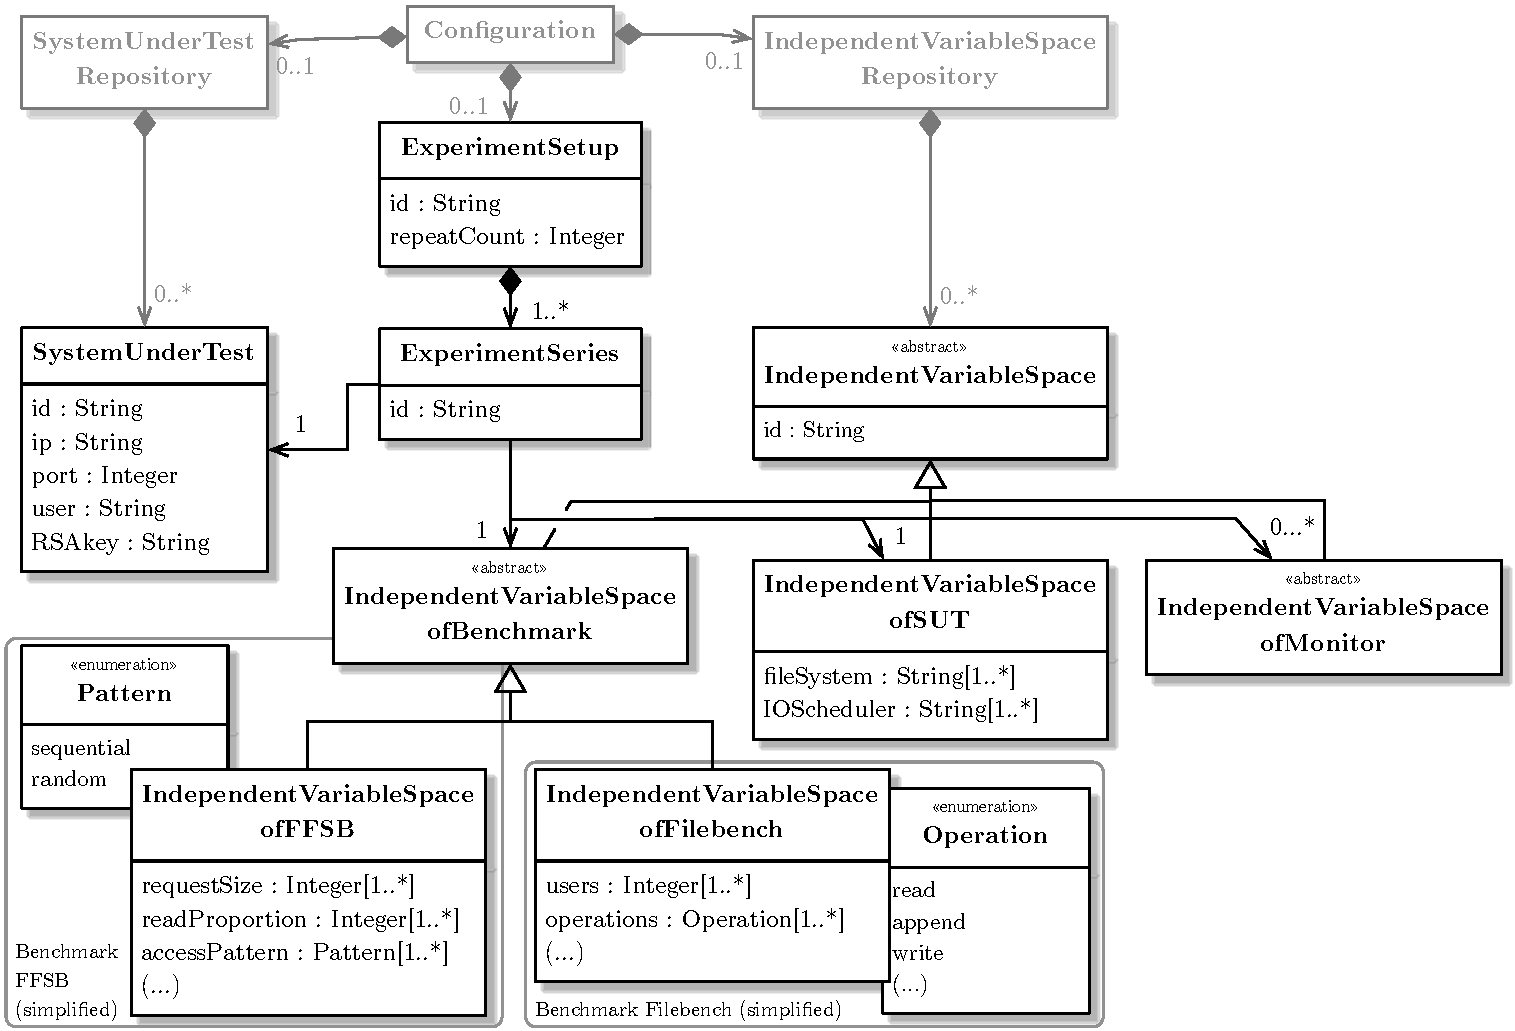
\includegraphics[scale=0.55]{graphics/DataModel.pdf}
    \caption{Configuration Model}
    \label{fig:DataModel}
\end{figure}

\section{Benchmark Configurations}

The configuration of a benchmark is defined in the respective \texttt{IndependentVariableSpaceofBenchmark} instances. For full details, please refer to the help files of the benchmarks. It is important to note that the \texttt{IndependentVariableSpaceofBenchmark} instances do only allow to configure a subset of all possible configuration possibilities since the benchmarks themselves do not necessarily support all configurations they actually allow. The configurations are therefore limited to either the most interesting or the best tested ones. However, there is no inherent limitation such that the configurations and the \texttt{BenchmarkDriver}s can be extended for other parameters.

For creating new configurations, please study the examples provided with the tool and compare your configurations with the actual benchmarks using their raw file output. You can also use the \texttt{Validate} option of the Eclipse tree editor to identify configuration errors. 

\textbf{Hint:} While the configuration units of Filebench can be passed, the units of FFSB configurations have been fixed for the sake of simplicity. They are \textit{bytes} for \texttt{(read|write)BlockSize}, \textit{kilobytes} for \texttt{fileSize}, and \textit{megabytes} for \texttt{fileSetSize}. The FFSB \texttt{BlockSize} (request size) can be either specified for both read and write separately, or for both combined using the parameters without 'read' or 'write' pre-/postfix.  
  

\chapter{Running the Benchmark}
After the configuration process has been completed and the configuration file is
finished, the benchmark can be started. This is done using the \texttt{run}
command in the \texttt{StorageBenchmarkHarness} directory. This command should
be executed in a terminal window as the application outputs all relevant
information on the standard out. The \texttt{run} command needs the following
parameters:
\begin{itemize*}
    \item \texttt{-c} or \texttt{--conf}: An absolute path to the configuration file which should be
        run. This configuration must contain a \textit{Experiment Setup} as
        explained above.
    \item \texttt{-d} or \texttt{--database}: An absolute path to the database
        file which should be used to save the results. If the database does not
        exist, an empty database is created.
\end{itemize*}
For additional parameters and their meaning see the output of the help screen or
the source code.

\section{Additional Output Files}
The Storage Benchmark Harness automatically parses and transforms the output of
the benchmarks into the database. If for debugging purposes or because
additional processing should be done later one the raw output of the benchmarks
should be saved, the \texttt{-r} or \texttt{--rawfilesavedir} parameter for the
\texttt{run} command can be used. This parameter should contain a directory in
which the raw files will be saved during the benchmarking. The user must pay
attention to the additional space which is necessary to store these files.

\section{Examples}
An example of a full command to run an experiment setup would look similar to this: 
\begin{lstlisting}
filebenchtargetdir=/mnt/noorsh \
./run -c ./configs/BenchmarkConfiguration.xmi \
-d ./results/database.sqlite \
-r ./results_raw/ \
| tee -a ./logs/spa.log
\end{lstlisting}

The results are stored in an SQLite database. Many operating system provide native command line access, for example on Mac OS, the statement to connect to the database would look similar to this:
\begin{lstlisting}
 $ sqlite3 ./results/database.sqlite
\end{lstlisting}

To show the available tables simply use the following command (more help is available at \url{http://www.sqlite.org/sqlite.html}):
\begin{lstlisting} 
 sqlite> .tables;
\end{lstlisting}

An even more convenient access is provided by the R libraries.

\chapter{R Libraries}

\section{Introduction}
\label{sec:RLIbraries:Introduction}

For the analysis of measurement results, a set of tailored libraries for the widely accepted statistics tool \emph{R}\footnote{\url{http://www.r-project.org/}}\footnote{\url{http://www.rstudio.com/}} have been developed. The starting point is the file \texttt{SPA.r} that loads all other libraries and a few examples automatically. These files build upon other standard libraries that can be installed automatically in a batch by using \texttt{installPackages.r} (simply load it using \texttt{source("filename")}).

\section{Interface}

The following parts contain the main functions and are loaded automatically in \texttt{SPA.r}\footnote{\textit{Hint:} Both the GUI and command line version of R allow auto completion with single/double \texttt{TAB} key.}. For more information, the functions are also commented directly in code.
\begin{itemize}
  \item \texttt{DataStoreInterface.r}: Loads the measurement data from the database.
  \begin{itemize}
    \item \texttt{getAllFFSBVars(db, metric=NULL, type=NULL)}
    \item \texttt{getAllFilebenchVars(db, metric=NULL, type=NULL)}
    \item[] Get the measurement data from the database located at \texttt{db} (path). Optionally, filter for certain metrics or result types. This can be specified using the \texttt{SPAMETRICCONSTANTS} and \texttt{SPATYPECONSTANTS} constant containers, respectively.
  \end{itemize}
  \item \texttt{RegressionOptimization.r}: Optimizes for given measurement data, in- and dependent variables the configuration for the regression techniques. 
  \begin{itemize}
    \item \texttt{optimizeTechniques(method, formula, data, ranges=NA, nSplits,} \texttt{nExplorations, trace=0, fold=NA, nIterations=15)} 
    \item[] Optimizes the \texttt{method} (``rpart'', ``earth'', ``,m5'', or ``cubist'') according to a \texttt{formula} using the given \texttt{data}. Optionally, the \texttt{ranges} of the method can be specified. Parameters of the optimization algorithm have the prefix ``\texttt{n}'', for details refer to~\cite{noorshams2013a}. The algorithm is deterministic if a \texttt{fold} for the cross-validation (objective function) is passed. Verbose output for \texttt{trace} = 1 or 2.
  \end{itemize}
  \item \texttt{RegressionModeling.r}: Creates the regression models either with a given configuration or in batch for comparing the models.
  \begin{itemize}
    \item \texttt{fitCertainModel(formula, data, method, parameter)}
    \item[] Use the \texttt{parameter}s obtained with \texttt{optimizeTechniques()} or specify others to create a model of the form given in \texttt{formula} with the \texttt{data} and the specific \texttt{method}.
    \item \texttt{fitModels<-function(formula, data, methods=list())}
    \item[] Alternatively, create a set of models of the form given in \texttt{formula} with the \texttt{data} with different methods and parameters to compare them. Optionally, a list of \texttt{methods} can be passed to create more models.
  \end{itemize}
\end{itemize}

\section{Examples}
\label{ch:RLIbraries:Examples}

\begin{lstlisting} 
 > # you can use setwd(path) to switch the working directory
 > # Copy-paste of these lines will not work because of special 
     symbols in the following such as quotes and tilde
 > source("installPackages.r")
 > source("SPA.r")
 > # The following example measurements are loaded automatically:
 > filebenchexample = getAllFilebenchVars("data/test/sqlite/
     filebenchtest.sqlite");
 > ffsbexample = getAllFFSBVars("data/test/sqlite/
     ffsbtest.sqlite", type=SPATYPECONSTANTS$mean);
 >
 > # example data provided by R (output abridged)
 > trees
    Girth Height Volume
 1:   8.3     70   10.3
 2:   8.6     65   10.3
 (...)
30:  18.0     80   51.0
31:  20.6     87   77.0
 >
 > # model with method EARTH
 > model = fitCertainModel(Volume~Girth+Height, trees, "earth", 
     parameter=data.table("nprune"=3, "nk"=3, 
     "degree"=1, "thresh"=0))     
> summary(model, digits = 2, style = "pmax") # output abridged 
Call: (...)
y =
  30
  + 6.6 * pmax(0, Girth -    14) 
  - 3.5 * pmax(0,    14 - Girth) 

Selected 3 of 3 terms, and 1 of 2 predictors 
Importance: Girth, Height-unused
Number of terms at each degree of interaction: 1 2 (...)
GCV 14    RSS 313    GRSq 0.95    RSq 0.96
 > plotmo(model$finalModel)

 grid:    Girth Height
           12.9     76
 >
 > # another method: RPART
 > model = fitCertainModel(Volume~Girth+Height, trees, "rpart", 
     parameter=data.table("cp"=0.01, "minsplit"=5))
 > plotCART(model$finalModel)
 >
 > # optimize the parameters
 > Eopt = optimizeTechniques(formula=Volume~Girth+Height, 
     data=trees, method="rpart",nIterations=3, nExplorations=2, 
     nSplits=3, trace=2)
 > modelOPT = fitCertainModel(Volume~Girth+Height, trees, 
     "rpart", parameter=Eopt)
 > plotCART(modelOPT$finalModel)
 >
 > # Create a set of models to compare the techniques 
 > models = fitModels(Volume~Girth+Height, trees) 
     # (output abridged)
Creating Fold
(...)
Training M5.
Calculating resamples.
 > summary(models$compare) # (output abridged)
(...)
MAPE 
                 Min. 1st Qu. Median   Mean 3rd Qu.  Max. NA's
lm              1.310   4.915  9.378 12.690  14.240 38.04    0
lm_2param_inter 2.651   5.794  6.215  7.408   9.744 13.75    0
(...)
m5              1.037   5.093  8.526 12.150  14.170 35.43    0

\end{lstlisting}


\chapter{Minimal Running Example}
\label{ch:MinimalRunningExample}

In this example, User \texttt{noorsh} runs FFSB on machine \texttt{IOMeasurements01} using RSA key \texttt{id\_rsa\_IOMeasurements01}. The controller machine is Mac OS (shown briefly is the execution of the controller on a Debian Linux system), the measurement target is Debian Linux.

\section{System Under Test Setup}

As described in Section~\ref{sec:Setup} and illustrated in Figure~\ref{fig:ExampleSUT}, ensure the user can connect to the system using RSA key without password prompt. And, as a minimal configuration, ensure FFSB is installed on the SUT and the binaries are in the user path, which can be checked using \texttt{which ffsb}. Root rights are only needed if the device scheduler should be modified.

\begin{figure}[htbp]
	\centering
	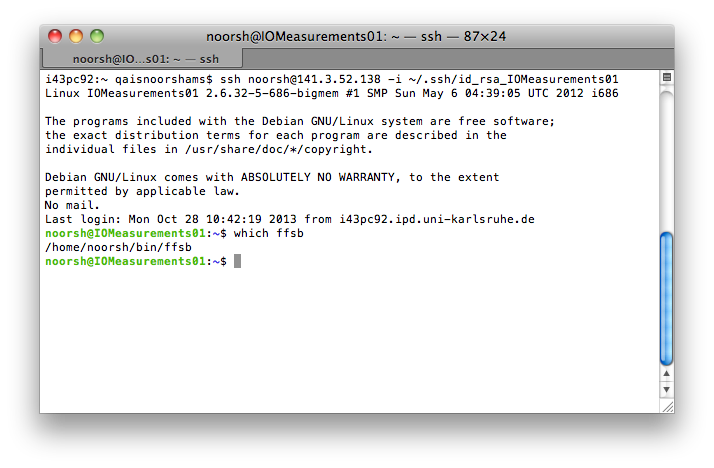
\includegraphics[scale=0.375]{graphics/example/SUT.png}
	\caption{Connection to the SUT}
 	\label{fig:ExampleSUT}
\end{figure}

\section{Installation and Compilation}

Download Eclipse Modeling Tools and import the SPA projects, cf. Figure~\ref{fig:ExampleImport}.

\begin{figure}[htbp]
	\centering
	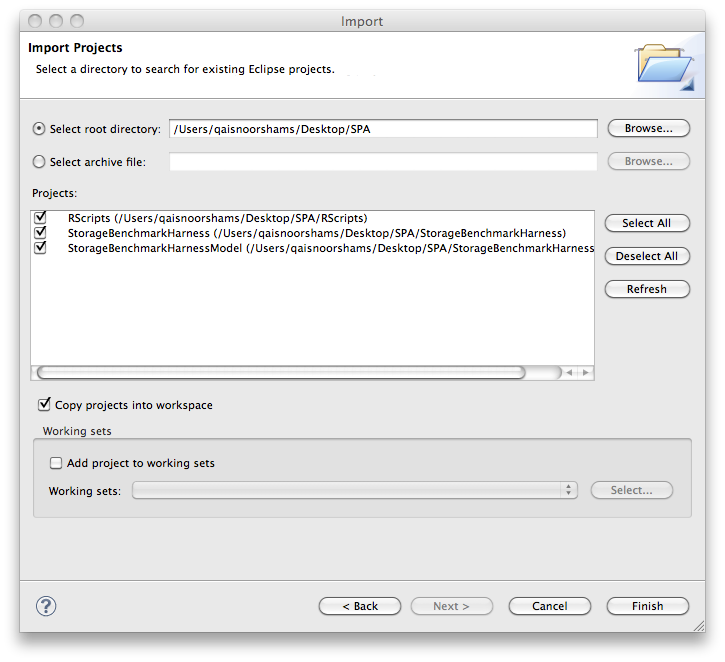
\includegraphics[scale=0.375]{graphics/example/Import.png}
	\caption{Import projects into Eclipse Modeling Tools}
 	\label{fig:ExampleImport}
 	\vspace{-8pt}
\end{figure}

After the import, you might get compilation errors and need to generate the EMF model code as shown in Figure~\ref{fig:ExampleGenerate} using \texttt{StorageBenchmarkHarnessModel/model/SBHModel.genmodel -> package context menu -> Generate All} (skip this step if the model code was already generated). Three new projects will be generated and all errors will disappear after a second if the project is rebuilt. In case the errors won't disappear, check the built path of the project \texttt{StorageBenchmarkHarnessModel} (\texttt{project context menu -> Properties -> Java Build Path}).

\begin{figure}[htbp]
	\centering
	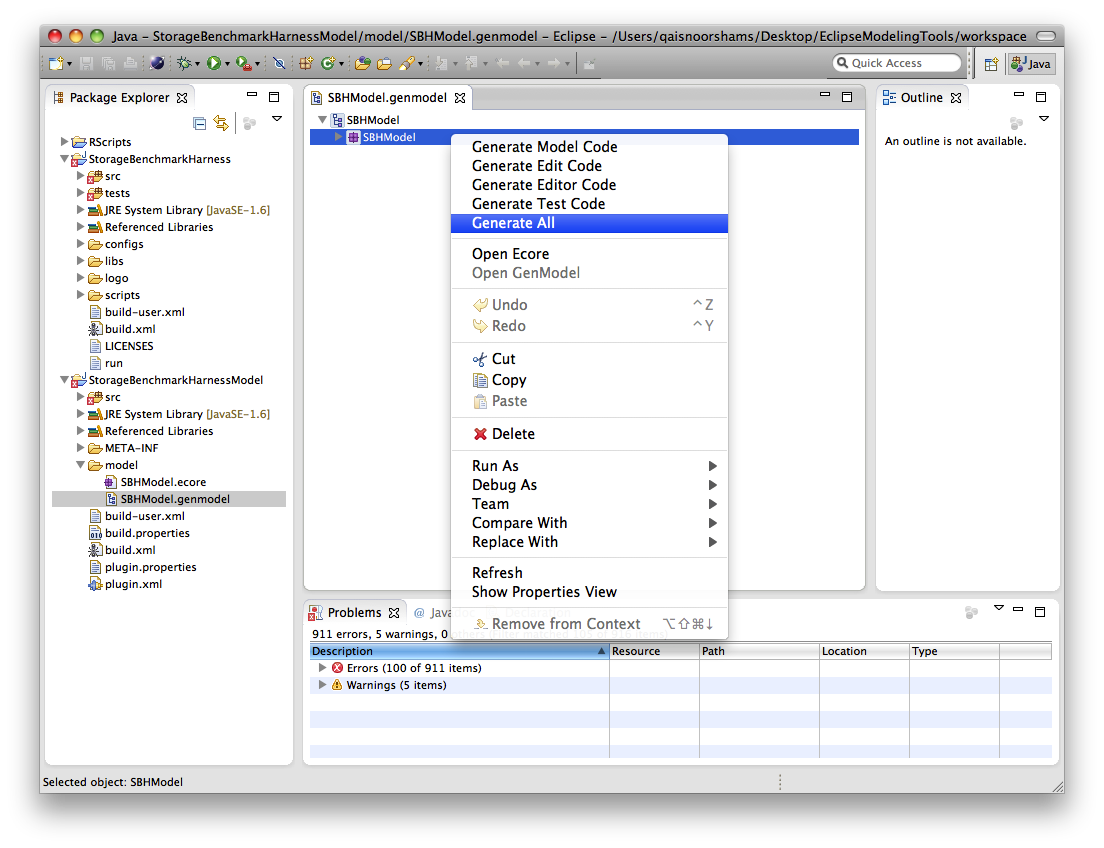
\includegraphics[scale=0.375]{graphics/example/Generate.png}
	\caption{Generate EMF model code using a genmodel}
 	\label{fig:ExampleGenerate}
\end{figure}

To easily manage the configuration files, install all plugins into the host as described in Section~\ref{sec:configurationfilecreation} and shown in Figure~\ref{fig:ExamplePlugins}.

\textbf{IMPORTANT:} If the projects are installed into the host, Eclipse may delete the \texttt{build.xml} file in the \texttt{StorageBenchmarkHarnessModel} project. Simply save it and re-import the file if a manual rebuild is necessary.

\begin{figure}[htbp]
	\centering
	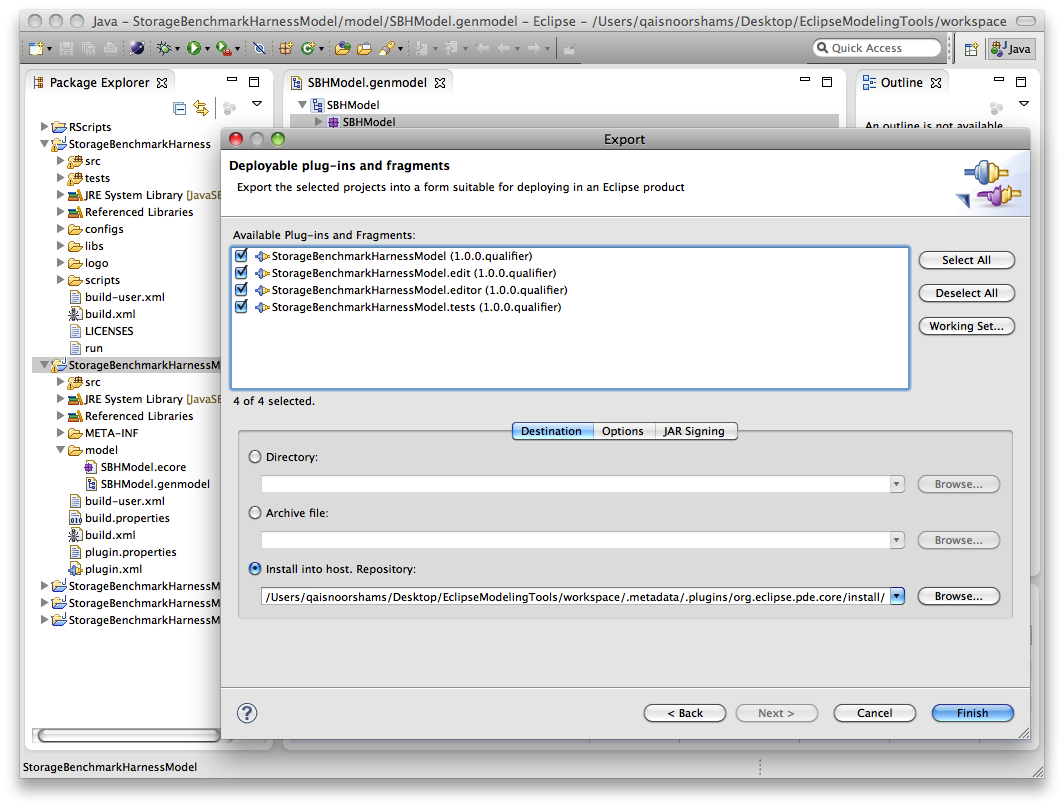
\includegraphics[scale=0.375]{graphics/example/Plugins.png}
	\caption{Install plugin projects into the host}
 	\label{fig:ExamplePlugins}
\end{figure}

You will now be able to open SPA configurations, e.g., located in \texttt{StorageBenchmarkHarness/configs/examples}, in the tree-based editor as shown in Figure~\ref{fig:ExampleConfiguration}. 

\begin{figure}[htbp]
	\centering
	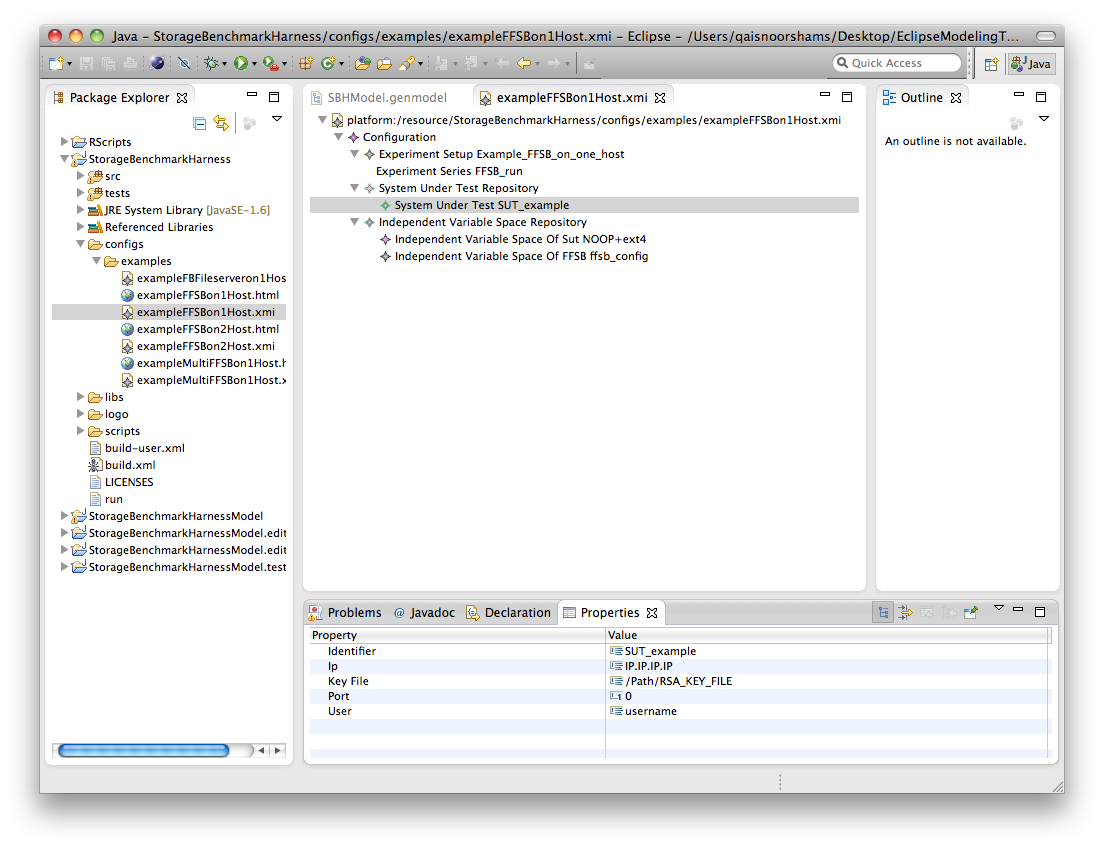
\includegraphics[scale=0.375]{graphics/example/Configuration.png}
	\caption{Example configuration in the tree-based editor}
 	\label{fig:ExampleConfiguration}
\end{figure}

You can execute the configurations using Eclipse run configuration or headless on the command line. For the former, open the \texttt{BenchmarkController} class in the package \texttt{edu.kit.sdq.storagebenchmarkharness} and click the run icon in order to execute the \texttt{main} method, cf. Figure~\ref{fig:ExampleRunEclipse}. For the latter, navigate to the \texttt{StorageBenchmarkHarness} project and execute \texttt{ant} if the project was not yet built automatically by Eclipse. The project can be run using \texttt{./run}, cf. Figure~\ref{fig:ExampleRunHeadless}. Either the Eclipse console or the command line will print the help.

\textbf{IMPORTANT:} If the projects were installed into the host, Eclipse may have deleted the \texttt{build.xml} file in the \texttt{StorageBenchmarkHarnessModel} project. Simply re-import the file if the project should be rebuilt manually.

\begin{figure}[htbp]
	\centering
	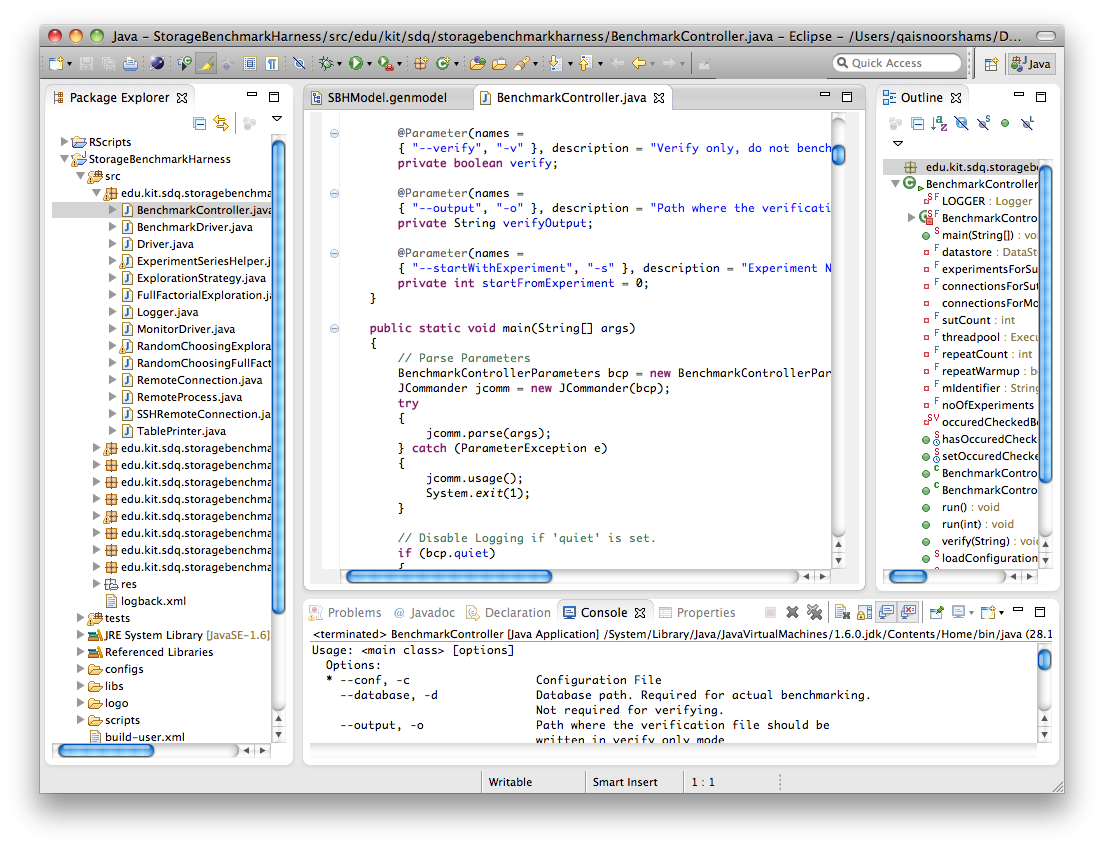
\includegraphics[scale=0.375]{graphics/example/RunEclipse.png}
	\caption{Run SPA in Eclipse}
 	\label{fig:ExampleRunEclipse}
\end{figure}

\begin{figure}[htbp]
	\centering
	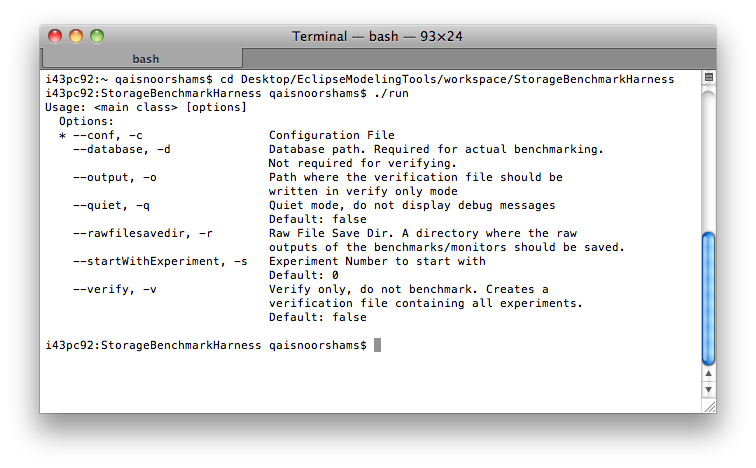
\includegraphics[scale=0.375]{graphics/example/RunHeadless.png}
	\caption{Run SPA in the terminal}
 	\label{fig:ExampleRunHeadless}
\end{figure}

\textbf{NOTE:} The code generation with Eclipse does only have to be done once. If this is done, the projects \texttt{StorageBenchmarkHarness} and \texttt{StorageBenchmarkHarnessModel} can be copied elsewhere and built and run headlessly, cf. Figure~\ref{fig:ExampleRunRemote}. 

\begin{figure}[htbp]
	\centering
	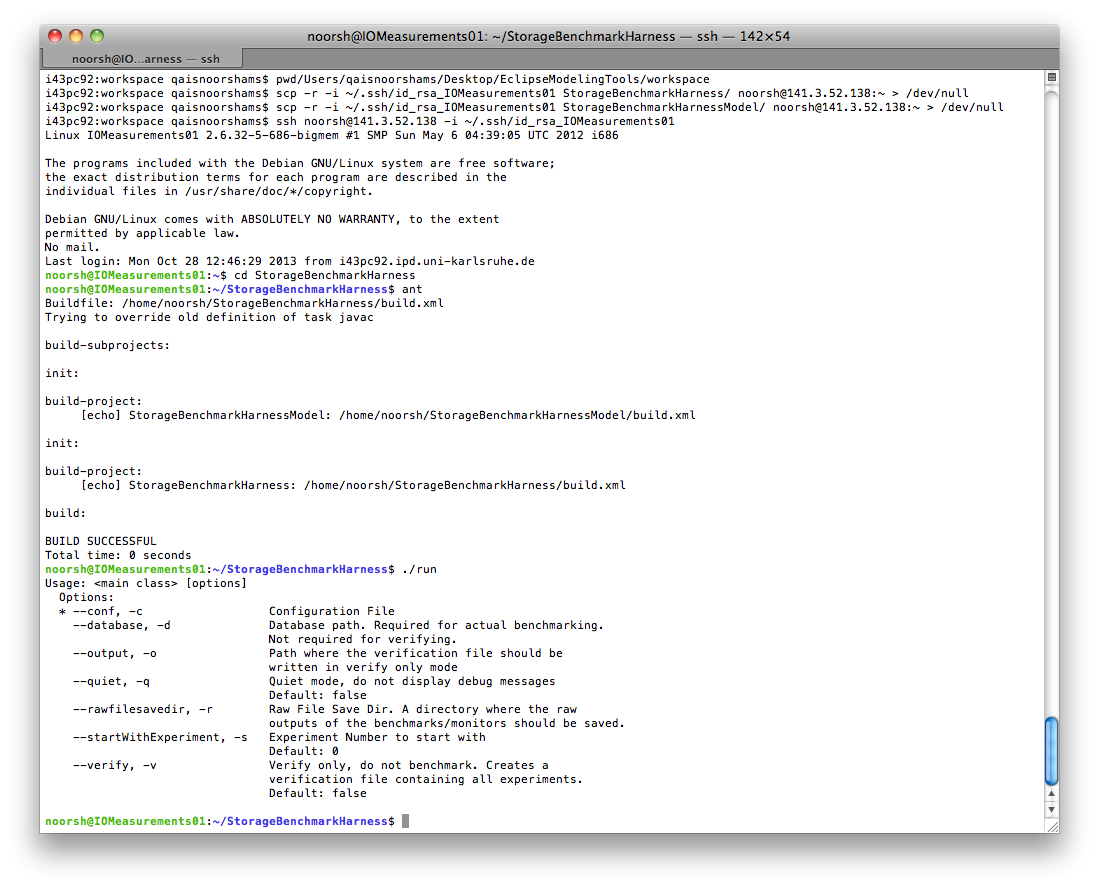
\includegraphics[scale=0.375]{graphics/example/RunRemote.png}
	\caption{Build and run SPA remotely}
 	\label{fig:ExampleRunRemote}
\end{figure}

\section{Configuration}

SPA configurations can be created using the tree-based editor of Eclipse. Eclipse can also check if a configuration is correct using the \texttt{validate} in the context menu. In the example, modify the \texttt{System Under Test} configuration of \texttt{StorageBenchmarkHarness/{\allowbreak}configs/examples/exampleFFSBon1Host.xmi} using the properties view. If the properties view is not shown by default, right-click on a given configuration element and choose \texttt{Show Properties View}. Change the SUT configuration according to your setup. In the example, the configuration looks as shown in Figure~\ref{fig:ExampleConfigurationSUT} (note that the key file is the \textit{private key}). You can check the configuration using the root element \texttt{Configuration -> right-click -> Validate}, which should give you no error.

\begin{figure}[htbp]
	\centering
	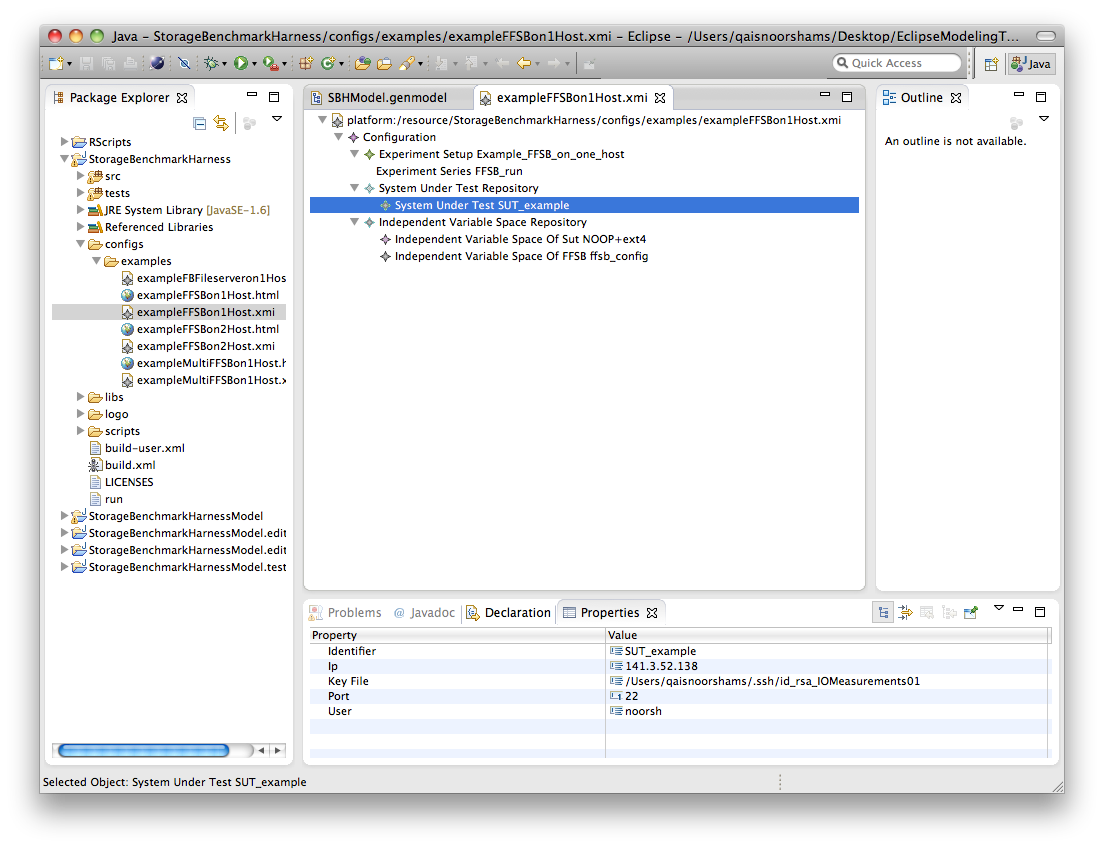
\includegraphics[scale=0.375]{graphics/example/ConfigurationSUT.png}
	\caption{SUT configuration in the example}
 	\label{fig:ExampleConfigurationSUT}
\end{figure}

\section{Running the Benchmark}

As described above, the benchmark can be compiled and executed using Eclipse or the command line. 
Using the Eclipse run configuration, you set the program arguments using the \texttt{Arguments} tab and set the environment variables in the \texttt{Environment} tab. Using the command line, you can set environment variables preceding \texttt{./run} and program arguments after.  
Both methods are the same, so in the examples we will only show the usage in the command line. 
To see what the example configuration would benchmark, on the command line use \texttt{./run -c configs/examples/exampleFFSBon1Host.xmi -v -o exampleFFSBon1Host.html}. Open the newly created file \texttt{exampleFFSBon1Host.html} to see the table contains 1 line and 1 column \texttt{SUT\_example} meaning that 1 experiment will be executed on the host \texttt{SUT\_example}.

To run the configuration, use \texttt{ffsbtargetdir=/mnt/noorsh/ffsb/ ./run -c configs/{\allowbreak}examples/exampleFFSBon1Host.xmi -d exampleFFSBon1Host.sqlite -r raw|tee exampleFFSBon1Host.log} to benchmark at the location \texttt{/mnt/noorsh/ffsb/} of the SUT using the configuration \texttt{exampleFFSBon1Host.xmi} and save the results in the database \texttt{exampleFFSBon1Host.sqlite} as well as the raw files in the folder \texttt{raw}. Additionally, save the run output into \texttt{exampleFFSBon1Host.log}. 

\textbf{IMPORTANT:} Make sure the scheduler of the target device is the same as specified in the configuration file in the \texttt{Independent Variable Space of SUT}, which is \texttt{NOOP} in the example, cf. Figure~\ref{fig:ExampleConfigurationSUT}. The scheduler can be checked using \texttt{cat /sys/block/[DEVICE]/queue/{\allowbreak}scheduler}.

The log of the benchmark in the raw folder will look like this (abridged): 

\begin{lstlisting}
FFSB version 6.0-RC2~fork started

benchmark time = 60
ThreadGroup 0
================
	 num_threads      = 10
	
	 read_random      = on
	 read_size        = 1048576	(1MB)
	 read_blocksize   = 4096	(4KB)
	 read_skip        = off
	 read_skipsize    = 0	(0B)
	
	 write_random     = on
	 write_size       = 1048576	(1MB)
	 fsync_file       = 0
	 write_blocksize  = 4096	(4KB)
	 wait time        = 0
	
	 op weights
	                 read = 100 (100.00%)
	              readall = 0 (0.00%)
	                write = 0 (0.00%)
	               create = 0 (0.00%)
	               append = 0 (0.00%)
	               delete = 0 (0.00%)
	               metaop = 0 (0.00%)
	            createdir = 0 (0.00%)
	                 stat = 0 (0.00%)
	             writeall = 0 (0.00%)
	       writeall_fsync = 0 (0.00%)
	           open_close = 0 (0.00%)
	          write_fsync = 0 (0.00%)
	         create_fsync = 0 (0.00%)
	         append_fsync = 0 (0.00%)
	
FileSystem /mnt/noorsh/ffsb/983bd7d3-a8a1-4122-95e4-f90c0ad81d5a
==========
	 num_dirs         = 100
	 starting files   = 64
	
	 min file size    = 16777216	(16MB)
	 max file size    = 16777216	(16MB)
	 directio         = on
	 alignedio        = on
	 bufferedio       = off
	
	 aging is off
	 current utilization = 15.95%
	
checking existing fs: /mnt/noorsh/ffsb/983bd7d3-a8a1-4122-95e4-f90c0ad81d5a
fs setup took 0 secs
Syncing()...0 sec
Starting Actual Benchmark At: Mon Oct 28 14:46:13 2013

Syncing()...0 sec
FFSB benchmark finished   at: Mon Oct 28 14:47:15 2013

Results:
Benchmark took 61.55 sec

Total Results
===============
             Op Name   Transactions	 Trans/sec	% Trans	    % Op Weight	   Throughput
             =======   ============	 =========	=======	    ===========	   ==========
                read :        99072	   1609.66	100.000%		100.000%	   6.29MB/sec
-
1609.66 Transactions per Second

Throughput Results
===================
Read Throughput: 6.29MB/sec

System Call Latency statistics in millisecs
=====
		Min		Avg		Max		Total Calls
		========	========	========	============
[   open]	0.004000	0.015760	0.052000	         387
   -
[   read]	0.163000	6.148361	228.093000	       99072
   -
[  lseek]	0.000000	0.001050	0.049000	       99072
   -
[  close]	0.002000	0.006049	0.014000	         387
   -

Discrete overall System Call Latency statistics in millisecs
=====

Overall Calls: 198918
=====
Values[ms]:
====
[   open]	Total calls:          387

0.012000
0.020000
(...) 
(Single Value Output)
(...)
====
[   stat]	Total calls:            0



0.2% User   Time
2.5% System Time
2.7% CPU Utilization
\end{lstlisting}

The log output of SPA will look like this (abridged), interesting are mostly the first and the last few lines:
\begin{lstlisting}
14:47:13.178 [main      ] DEBUG e.k.s.s.d.s.SQLiteDataStore    - Opening Database 'exampleFFSBon1Host.sqlite'
14:47:13.208 [SQLiteQueu] DEBUG e.k.s.s.d.s.SBHSQLiteQueue     - Starting executing Job SQLiteDataStore$1@6f878144
14:47:13.211 [SQLiteQueu] DEBUG e.k.s.s.d.s.SBHSQLiteQueue     - Finished executing Job SQLiteDataStore$1@6f878144
14:47:13.225 [main      ] DEBUG e.k.s.s.BenchmarkController    - Reading Configuration from configs/examples/exampleFFSBon1Host.xmi
14:47:13.759 [main      ] DEBUG e.k.s.s.BenchmarkController    - Validating Objects:
14:47:13.775 [main      ] DEBUG e.k.s.s.BenchmarkController    - Validating edu.kit.sdq.storagebenchmarkharness.SBHModel.Configuration.Configuration@508aeb74
(...)
(Validating Objects)
(...)
14:47:14.865 [main      ] DEBUG e.k.s.s.BenchmarkController    - Setup is edu.kit.sdq.storagebenchmarkharness.SBHModel.Configuration.ExperimentSetup@6e82254d (identifier: Example_FFSB_on_one_host, repeatCount: 1, repeatWarmup: false)
14:47:14.865 [main      ] DEBUG e.k.s.s.BenchmarkController    - Found series edu.kit.sdq.storagebenchmarkharness.SBHModel.Configuration.ExperimentSeries@225f1ae9 (identifier: FFSB_run)
14:47:14.866 [main      ] DEBUG e.k.s.s.BenchmarkController    - No connection found for SUT SUT_example, creating one
14:47:14.868 [main      ] DEBUG e.k.s.s.SSHRemoteConnection    - Creating remote connection to edu.kit.sdq.storagebenchmarkharness.SBHModel.Configuration.SystemUnderTest@3f3a0212 (identifier: SUT_example, ip: 141.3.52.138, port: 22, user: noorsh, keyFile: /Users/qaisnoorshams/.ssh/id_rsa_IOMeasurements01)
14:47:14.869 [main      ] DEBUG e.k.s.s.BenchmarkController    - No connection set found for monitoring the SUT SUT_example, creating one
14:47:14.869 [main      ] DEBUG e.k.s.s.BenchmarkController    - Adding Experiments
14:47:14.875 [main      ] DEBUG e.k.s.s.BenchmarkDriver        - RawFileSaveDir is raw
14:47:14.908 [main      ] DEBUG e.k.s.s.b.f.FFSBenchmarkDriver - TargetDir is /mnt/noorsh/ffsb/
14:47:14.908 [main      ] DEBUG e.k.s.s.ExperimentSeriesHelper - Expanding series edu.kit.sdq.storagebenchmarkharness.SBHModel.Configuration.ExperimentSeries@225f1ae9 (identifier: FFSB_run)
14:47:14.908 [main      ] DEBUG e.k.s.s.ExperimentSeriesHelper - Creating SUTVariables
14:47:14.910 [main      ] DEBUG e.k.s.s.ExperimentSeriesHelper - Creating BenchmarkVariables
14:47:14.912 [main      ] DEBUG e.k.s.s.BenchmarkController    - Found 1 Experiments in this series
14:47:14.914 [main      ] DEBUG e.k.s.s.d.s.SQLiteDataStore    - Setting up Database
14:47:14.914 [SQLiteQueu] DEBUG e.k.s.s.d.s.SBHSQLiteQueue     - Starting executing Job SQLiteDataStore$2@1343a083
14:47:14.928 [SQLiteQueu] DEBUG e.k.s.s.d.s.SQLiteHelper       - Create SQL ALTER TABLE ffsbIndependentVars ADD COLUMN fileSystem VARCHAR DEFAULT NULL;
(...)
(SQL Statements)
(...)
14:47:14.993 [SQLiteQueu] DEBUG e.k.s.s.d.s.SBHSQLiteQueue     - Finished executing Job SQLiteDataStore$2@1343a083
14:47:14.994 [main      ] DEBUG e.k.s.s.BenchmarkController    - Connecting to all SUTs:
14:47:14.999 [main      ] DEBUG e.k.s.s.SSHRemoteConnection    - Adding publickey /Users/qaisnoorshams/.ssh/id_rsa_IOMeasurements01
14:47:15.011 [main      ] DEBUG e.k.s.s.SSHRemoteConnection    - Connecting to 141.3.52.138:22
14:47:17.288 [SQLiteQueu] DEBUG e.k.s.s.d.s.SBHSQLiteQueue     - Starting executing Job SQLiteDataStore$3@d2f41a5
14:47:17.290 [SQLiteQueu] DEBUG e.k.s.s.d.s.SBHSQLiteQueue     - Finished executing Job SQLiteDataStore$3@d2f41a5
14:47:17.290 [main      ] DEBUG e.k.s.s.BenchmarkController    - Create connecting for monitoring
14:47:17.291 [main      ] DEBUG e.k.s.s.BenchmarkController    - Creating and starting Threads
14:47:17.293 [main      ] DEBUG e.k.s.s.BenchmarkController    - Waiting for Threads to finish
14:47:17.294 [H-SUT_exam] DEBUG e.k.s.s.BenchmarkController    - Configuration: edu.kit.sdq.storagebenchmarkharness.SBHModel.IndependentVariablesOfSut@21455cf0 (fileSystem: ext4, scheduler: NOOP)/edu.kit.sdq.storagebenchmarkharness.SBHModel.IndependentVariablesOfFFSB@50d8a1a0 (readPercentage: 100, blockSize: null, writeBlockSize: 4096, readBlockSize: 4096, filesetSize: 1024, sequentialAccess: null, sequentialRead: false, sequentialWrite: false, writeFsync: false, threadCount: 10, runTime: 60, warmUpTime: 30, fileSize: 16384, opsPerFile: 256, directIO: true, opsPerFileRead: null, opsPerFileWrite: null, opDelay: 0)
14:47:17.294 [H-SUT_exam] DEBUG e.k.s.s.BenchmarkController    - Waiting for barrier for preparation
14:47:17.294 [H-SUT_exam] DEBUG e.k.s.s.BenchmarkController    - Repeat 1/1
14:47:17.294 [H-SUT_exam] DEBUG e.k.s.s.BenchmarkController    - Preparing experiment
14:47:17.304 [H-SUT_exam] DEBUG e.k.s.s.SSHRemoteConnection    - Command is bash -l -c 'mkdir /mnt/noorsh/ffsb/983bd7d3-a8a1-4122-95e4-f90c0ad81d5a'
14:47:17.507 [H-SUT_exam] DEBUG e.k.s.s.b.f.FFSBenchmarkDriver - FFSB Configfile is /tmp/d3526247-d501-4501-90da-4b07cc4d3f07.warmup.ffsb and /tmp/d3526247-d501-4501-90da-4b07cc4d3f07.bench.ffsb
14:47:17.509 [H-SUT_exam] DEBUG e.k.s.s.SSHRemoteConnection    - Command is bash -l -c 'tee /tmp/d3526247-d501-4501-90da-4b07cc4d3f07.warmup.ffsb'
14:47:17.713 [H-SUT_exam] DEBUG e.k.s.s.SSHRemoteConnection    - Command is bash -l -c 'tee /tmp/d3526247-d501-4501-90da-4b07cc4d3f07.bench.ffsb'
14:47:17.921 [H-SUT_exam] DEBUG e.k.s.s.BenchmarkDriver        - Setting scheduler to NOOP
14:47:17.921 [H-SUT_exam] DEBUG e.k.s.s.SSHRemoteConnection    - Command is bash -l -c 'readlink -f `df -T -P /mnt/noorsh/ffsb/983bd7d3-a8a1-4122-95e4-f90c0ad81d5a | awk '\''NR>1 {printf $1}'\''`'
14:47:18.140 [H-SUT_exam] DEBUG e.k.s.s.SSHRemoteConnection    - Command is bash -l -c 'cat /sys/class/block/xvdb/queue/scheduler'
14:47:18.355 [H-SUT_exam] DEBUG e.k.s.s.BenchmarkDriver        - Available schedulers are [[noop], anticipatory, deadline, cfq, 
]
14:47:18.355 [H-SUT_exam] DEBUG e.k.s.s.BenchmarkDriver        - Scheduler noop is already active, doing nothing
14:47:18.356 [H-SUT_exam] DEBUG e.k.s.s.SSHRemoteConnection    - Command is bash -l -c 'df -T -P /mnt/noorsh/ffsb/983bd7d3-a8a1-4122-95e4-f90c0ad81d5a | awk '\''NR>1 {printf $2}'\'''
14:47:18.573 [H-SUT_exam] DEBUG e.k.s.s.BenchmarkDriver        - Current Filesystem ext4, expected ext4
14:47:18.573 [H-SUT_exam] DEBUG e.k.s.s.b.f.FFSBenchmarkDriver - FFSB Warmup
14:47:18.574 [H-SUT_exam] DEBUG e.k.s.s.SSHRemoteConnection    - Command is bash -l -c 'ffsb /tmp/d3526247-d501-4501-90da-4b07cc4d3f07.warmup.ffsb'
14:47:54.429 [H-SUT_exam] DEBUG e.k.s.s.BenchmarkController    - Waiting for start monitoring
14:47:54.429 [H-SUT_exam] DEBUG e.k.s.s.BenchmarkController    - Waiting for all monitors to be started
14:47:54.429 [H-SUT_exam] DEBUG e.k.s.s.BenchmarkController    - Starting Benchmarking
14:47:54.429 [H-SUT_exam] DEBUG e.k.s.s.b.f.FFSBenchmarkDriver - Executing FFSB for #1
14:47:54.430 [H-SUT_exam] DEBUG e.k.s.s.SSHRemoteConnection    - Command is bash -l -c 'ffsb /tmp/d3526247-d501-4501-90da-4b07cc4d3f07.bench.ffsb'
14:48:56.122 [H-SUT_exam] DEBUG e.k.s.s.b.f.FFSBenchmarkDriver - Found Main Heading
14:48:56.123 [H-SUT_exam] DEBUG e.k.s.s.b.f.FFSBenchmarkDriver - Found Heading open
14:48:56.131 [H-SUT_exam] DEBUG e.k.s.s.b.f.FFSBenchmarkDriver - Found Heading read
14:48:57.281 [H-SUT_exam] DEBUG e.k.s.s.b.f.FFSBenchmarkDriver - Found Heading write
14:48:57.282 [H-SUT_exam] DEBUG e.k.s.s.b.f.FFSBenchmarkDriver - Found Heading create
14:48:57.282 [H-SUT_exam] DEBUG e.k.s.s.b.f.FFSBenchmarkDriver - Found Heading lseek
14:48:57.994 [H-SUT_exam] DEBUG e.k.s.s.b.f.FFSBenchmarkDriver - Found Heading unlink
14:48:57.994 [H-SUT_exam] DEBUG e.k.s.s.b.f.FFSBenchmarkDriver - Found Heading close
14:48:57.997 [H-SUT_exam] DEBUG e.k.s.s.b.f.FFSBenchmarkDriver - Found Heading stat
14:48:58.017 [H-SUT_exam] DEBUG e.k.s.s.BenchmarkController    - Waiting for finishing of benchmarking
14:48:58.017 [H-SUT_exam] DEBUG e.k.s.s.BenchmarkController    - Stopping monitors...
14:48:58.017 [H-SUT_exam] DEBUG e.k.s.s.BenchmarkController    - Finished Monitoring
14:48:58.017 [H-SUT_exam] DEBUG e.k.s.s.BenchmarkController    - Waiting to store results
14:48:58.017 [H-SUT_exam] DEBUG e.k.s.s.BenchmarkController    - Result-Storing-Phase: 1 Results in database
14:48:58.018 [H-SUT_exam] DEBUG e.k.s.s.BenchmarkController    - Results stored
14:48:58.018 [SQLiteQueu] DEBUG e.k.s.s.d.s.SBHSQLiteQueue     - Starting executing Job SQLiteDataStore$4@56ee20fe
14:48:58.018 [H-SUT_exam] DEBUG e.k.s.s.BenchmarkController    - Finishing Experiment
14:48:58.018 [H-SUT_exam] DEBUG e.k.s.s.BenchmarkController    - Waiting for finish
14:48:58.018 [H-SUT_exam] DEBUG e.k.s.s.BenchmarkController    - Finishing Experiment
14:48:58.018 [SQLiteQueu] DEBUG e.k.s.s.d.s.SQLiteDataStore    - Starting saving 99075 results for host SUT_example, expNo 0, repeatNo 1
14:48:58.018 [H-SUT_exam] DEBUG e.k.s.s.SSHRemoteConnection    - Command is bash -l -c 'rm /tmp/d3526247-d501-4501-90da-4b07cc4d3f07.bench.ffsb'
14:48:58.220 [H-SUT_exam] DEBUG e.k.s.s.SSHRemoteConnection    - Command is bash -l -c 'rm /tmp/d3526247-d501-4501-90da-4b07cc4d3f07.warmup.ffsb'
14:48:58.421 [H-SUT_exam] DEBUG e.k.s.s.SSHRemoteConnection    - Command is bash -l -c 'rm -r /mnt/noorsh/ffsb/983bd7d3-a8a1-4122-95e4-f90c0ad81d5a'
14:48:58.822 [main      ] DEBUG e.k.s.s.BenchmarkController    - All Threads for expNo 0 finished
14:48:58.822 [main      ] DEBUG e.k.s.s.BenchmarkController    - Finishing Cofiguration Run
14:48:59.050 [SQLiteQueu] DEBUG e.k.s.s.d.s.SQLiteDataStore    - Finished saving 99075 results for host SUT_example, expNo 0, repeatNo 1
14:48:59.050 [SQLiteQueu] DEBUG e.k.s.s.d.s.SBHSQLiteQueue     - Finished executing Job SQLiteDataStore$4@56ee20fe
14:48:59.050 [SQLiteQueu] DEBUG e.k.s.s.d.s.SBHSQLiteQueue     - Starting executing Job SQLiteDataStore$5@32b3a5a0
14:48:59.051 [main      ] DEBUG e.k.s.s.BenchmarkController    - Closing all connections
14:48:59.051 [SQLiteQueu] DEBUG e.k.s.s.d.s.SBHSQLiteQueue     - Finished executing Job SQLiteDataStore$5@32b3a5a0
14:48:59.053 [main      ] DEBUG e.k.s.s.BenchmarkController    - Closing all remaining connections
14:48:59.054 [main      ] DEBUG e.k.s.s.BenchmarkController    - Shutting down the threadpool
14:48:59.054 [main      ] DEBUG e.k.s.s.BenchmarkController    - Closing the datastore

\end{lstlisting} 

\section{R Libraries}

After all the required R packages are installed, cf. Section~\ref{sec:RLIbraries:Introduction}, the experiment results can be analyzed in R by loading the libraries and using the corresponding interface method (output abridged):

\begin{lstlisting}
 i43pc92:StorageBenchmarkHarness qaisnoorshams$ r
WARNING: ignoring environment value of R_HOME

R version 3.0.1 (2013-05-16) -- "Good Sport"
(...)
> getwd()
[1] "/Users/qaisnoorshams/Desktop/EclipseModelingTools/workspace/StorageBenchmarkHarness"
> source("../RScripts/SPA.r")
data.table 1.8.10  For help type: help("data.table")
(...)
Registering doMC parallel backend
> dat = getAllFFSBVars("exampleFFSBon1Host.sqlite",type=SPATYPECONSTANTS$mean)
> dat
   runId             crIdentifier              crTime repeatNo expNo
1:     1 Example_FFSB_on_one_host 2013-10-28 13:47:17        1     0
2:     1 Example_FFSB_on_one_host 2013-10-28 13:47:17        1     0
        hostId                               expUid fileSystem scheduler
1: SUT_example 2843dc71-fa5f-4098-b3ac-7b03129c58c6       ext4      NOOP
2: SUT_example 2843dc71-fa5f-4098-b3ac-7b03129c58c6       ext4      NOOP
   readPercentage writeBlockSize readBlockSize filesetSize sequentialRead
1:            100           4096          4096        1024              0
2:            100           4096          4096        1024              0
   sequentialWrite writeFsync threadCount runTime warmUpTime fileSize
1:               0          0          10      60         30    16384
2:               0          0          10      60         30    16384
   opsPerFile directIO opDelay dvId benchPrefix valueId operation     opMetric
1:        256        1       0    1        ffsb       1      read   throughput
2:        256        1       0    1        ffsb       2      read responseTime
    opValue opType
1: 6.290000   mean
2: 6.148361   mean
>
>
> dat[,list(opMetric,opValue)]
       opMetric  opValue
1:   throughput 6.290000
2: responseTime 6.148361
> 
> datSingle = getAllFFSBVars("exampleFFSBon1Host.sqlite",type=SPATYPECONSTANTS$singleValue)
> summary(datSingle[opMetric=='responseTime',opValue])
   Min. 1st Qu.  Median    Mean 3rd Qu.    Max. 
  0.163   0.705   3.873   6.148   8.101 228.100 
> 
\end{lstlisting}

The last commands show the results in brief, cf. benchmark log output above. One caveat is that the units are not transferred automatically and need to be considered while analyzing the results. 

A minimal example for the SPA modeling functions is shown in Section~\ref{ch:RLIbraries:Examples}.

\chapter{Questions \& Answers}

\Que{Why are forks of the benchmarks used instead of the official versions?}
\Ans{Both used benchmarks include bugfixes and FFSB also includes the extensions to capture single request measurements instead of just mean values. This allows, e.g., to also analyze the distribution of the measurements.}

\Que{Why does Filebench get restarted multiple times during the benchmark execution?}
\Ans{On several machines, Filebench seems to run unstably or freeze during the execution. The Benchmark Driver of Filebench is able to recognize a failed execution and restarts the benchmark automatically. This is why the execution of Filebench requires some root rights. This might result in a longer benchmarking period, but no manual interaction is required.}

\Que{What is the minimal setup to test the tool?}
\Ans{You need i) a password-less connection to the system you want to benchmark (using RSA) and ii) one benchmark installed (the executable needs to reside in the user path), cf. Section~\ref{sec:Setup}. Root rights are not required for FFSB (only if the I/O scheduler of the system needs to be changed). A minimal configuration contains an Experiment Setup with one Experiment Series specifying i) a System Under Test (SUT), ii) an Independent Variable Space of the SUT, and iii) an Independent Variable Space of the Benchmark, cf. Figure~\ref{fig:DataModel}. A minimal running example is shown in Section~\ref{ch:MinimalRunningExample}.} 

\Que{Why is/are the device/s on the System Under Test getting full?}
\Ans{Additionally to the log files, temporary files are stored in \texttt{/tmp}. If the experiments are interrupted due to errors, the files might not get cleaned up properly. Check the measurement and monitoring targets as well as \texttt{/tmp} for temporary files in case of interrupted runs.} 